\begin{frame}{Semi–infinite Slab}
    Given a hyperplane $P = \left\{\mathbf x \mid \mathbf n^\intercal \mathbf x = b\right\} \subset \mathbb R^n$. \textbf{A semi–infinite slab} defined by hyperplane $P$, is given by:
    \[
    Slab_\infty(P) \stackrel{\text{def}}{=} \left\{\mathbf x \in \mathbb R^n \mid \mathbf n^\intercal \mathbf x < b\right\}
    \]
    Indeed, it is a convex set \cite{boyd2004convex}.

    \begin{figure}[H]
        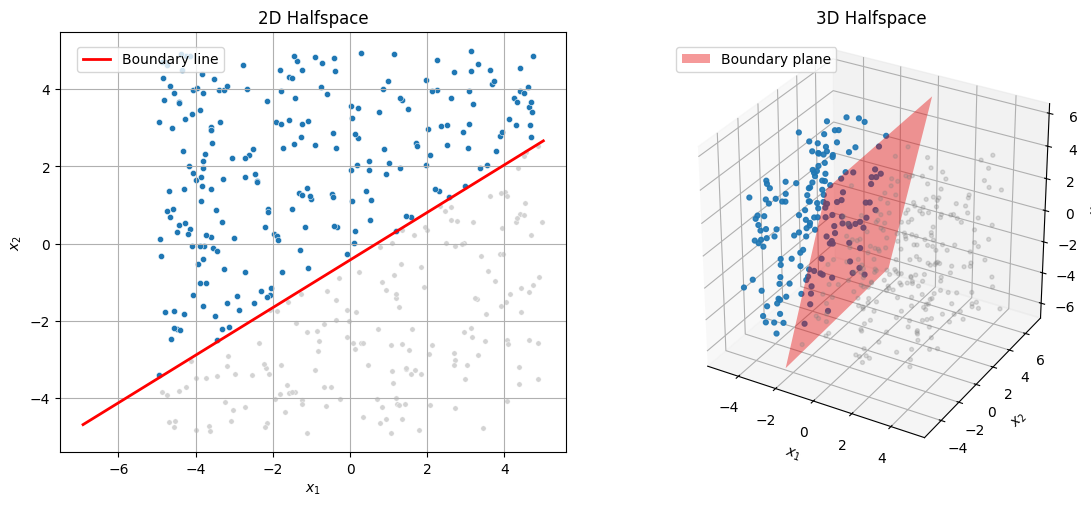
\includegraphics[width=0.9\textwidth]{figures/fig_13.png}
        \label{fig:fig_13}
    \end{figure}
\end{frame}